\section{Моделирование и оптимизация двухкубитных логических операций}
\label{sec:chapter_4}

\subsection{Ридберговская блокада}

\subsection{Последовательность Levine-Pichler, гейт CNOT}

\subsection{Моделирование двухфотонного ридберговского возбуждения}

\subsubsection{Тепловое движение атома в оптическом пинцете}

\subsubsection{Спонтанный распад из промежуточного состояния}

\subsubsection{Фазовые шумы лазера}

\subsubsection{Ошибки приготовления и измерения состояния}

\subsection{Измерение параметров модели}

\subsubsection{Гетеродинное измерение спектра фазовых шумов лазеров}


% \begin{figure}
% 	\centering
% 	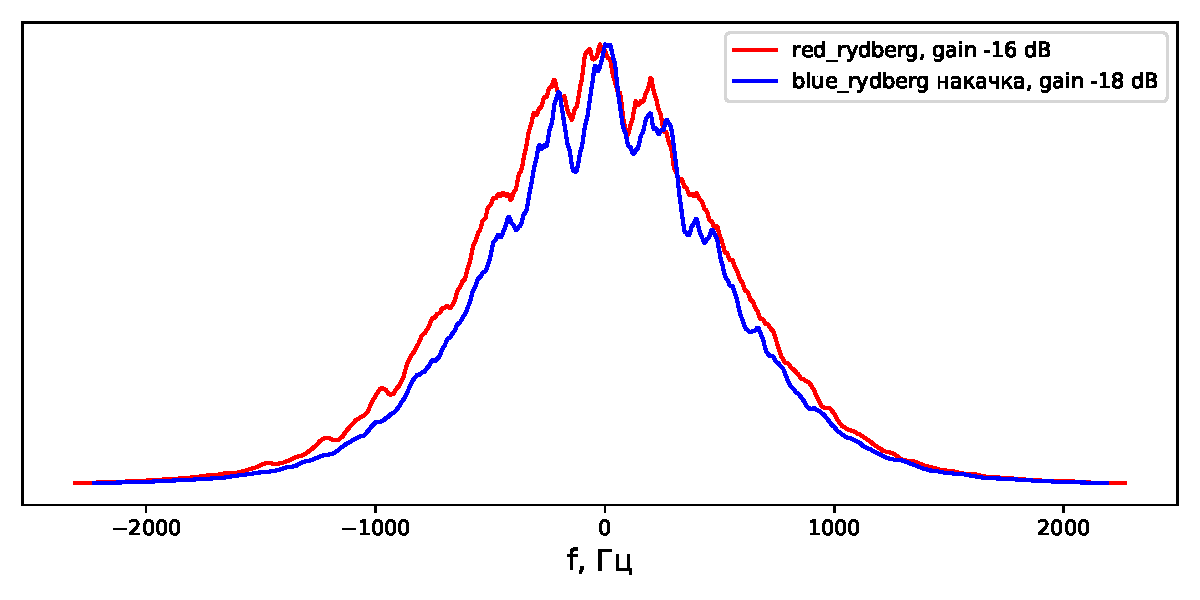
\includegraphics[width=0.75\textwidth]{images/turbo_spectrum.pdf}
% 	\caption{Спектры лазеров, используемых для двухфотонного ридберговского возбуждения при включенном турбонасосе.}
% 	\label{fig:turbo_spectrum}
% \end{figure}

\subsubsection{Измерение SPAM-ошибки}

\subsection{Улучшение двухкубитных вентилей за счёт flat-top пучков}

\subsection{Результаты главы}


\newpage